\section{Model Discussion}

As a part of the creation of our agent-based model, where numerous climate and regional factors contribute to the spread of dandelion plants, we found it essential to conduct a sensitivity analysis to determine the most impactful factors on dandelion growth. Beyond our sensitivity analysis, we also provide a brief discussion of our model's key strengths and weaknesses, as well as a scope of how our model can be readily generalizable to virtually any plot of land.

\subsection{Model Hyperparameters}

The following table consolidates all hyperparameters based on our model described above. Our sensitivity analysis therefore investigates the impacts of these hyperparameters on the spread of dandelion plants and seeds.

\begin{table}[h!]
\renewcommand{\arraystretch}{1.3}
%p{0.8\linewidth
    \begin{tabularx}{\textwidth}{p{0.18\textwidth}lp{0.45\textwidth}X}
    \toprule
    \textbf{Hyperparameter}  & \textbf{Symbol} & \textbf{Description} & \textbf{Default Value} \\ \midrule
    \raggedright Temperature & \(\tau(t)\)   & Temperature (\(^\circ\)F) over a year in a specific region. Dandelions grow optimally between \(50-77^\circ\) F \cite{noauthor_dandelion_nodate-2}. & Temperatures of Clay, NY (2022) \cite{aladin_wolcott_nodate}. \\
    \rowcolor{gray!15}
    \raggedright Light Levels & \(l(t)\)  & Hours of sunlight per day over a year. Dandelions grow best between 6-24 light hours per day \cite{stewart-wade_biology_2002}. & Daily hours of light of Clay, NY (2022) data \cite{aladin_wolcott_nodate}.\\
    \raggedright Wind Levels & \(m(t)\) & Average mph of wind per day over a year which affects movement processes. & Wind levels in Clay, NY (2022) \cite{aladin_wolcott_nodate}. \\
   \rowcolor{gray!15} \raggedright K Levels & \(k(t)\) & Average amount of potassium in a regionally collected sample of soil in ppm over time. K levels account for soil moisture and richness \cite{noauthor_potassium_nodate}. & K levels from a soil survey \cite{communications_interpreting_2018}.\\
      \raggedright N Levels & \(n(t)\) & Average amount of Nitrogen (ppm) over time in a regionally collected sample of soil. & N levels from a soil survey \cite{pritchett_nitrogen_1959}.\\
    \rowcolor{gray!15} \raggedright Seed Lifespan & \(\lambda_s(t)\) & Average time until death for dandelion seeds. & 4 days \cite{noauthor_dandelion_nodate}. \\
    \raggedright Dandelion Lifespan & \(\lambda_d(t)\) & Average time until death for dandelion plants. & 15 days \cite{farmshowGrowingDandelions}. \\
     \rowcolor{gray!15} \raggedright Initial Seeds & \(S_0\) & Number of seeds dispersed by each puffball. & 2000 seeds \cite{noauthor_dandelion_nodate-2}. \\
    \bottomrule
    \end{tabularx}
\end{table}

\subsection{Sensitivity Analysis}

A standard methodology for sensitivity analysis is to randomly sample various values and analyze the model's output. Therefore, to randomly examine different sets of hyperparameters for our model, we employed a Monte Carlo sampling simulation to randomly sample \(\pm 10\%\) of default values. Based on the simulation, we modeled the effects of these changes on the growth of dandelion plant populations over time. These results are shown in Figure~\ref{fig:sensitivitypopulation}.

\begin{figure}[h!]
\centering
    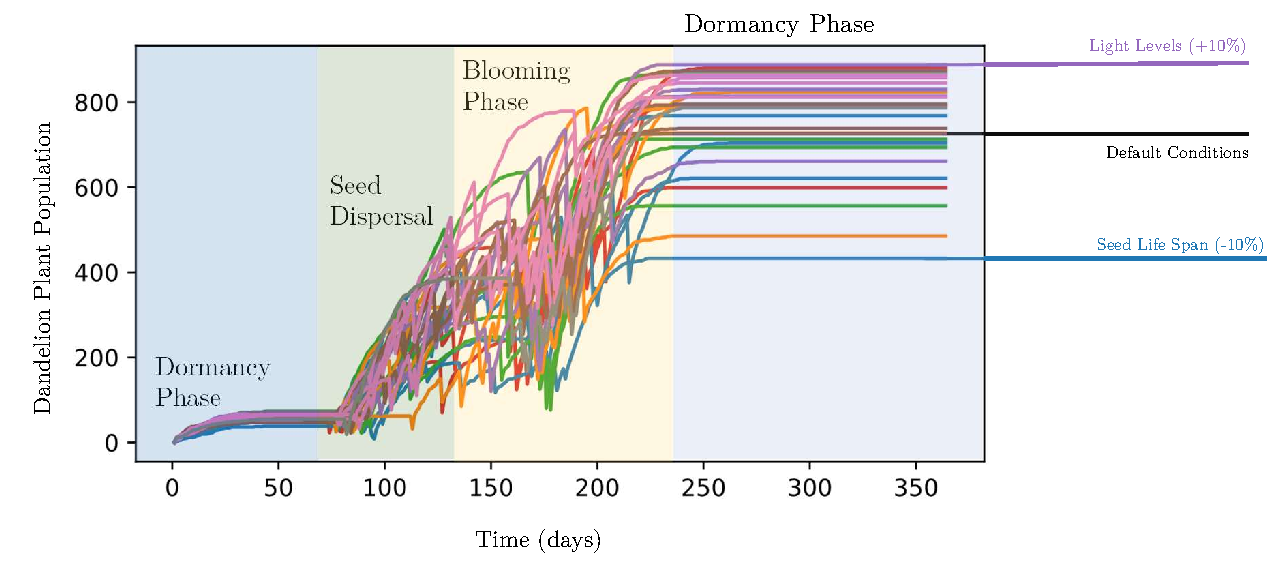
\includegraphics[scale=0.7]{figures/sensitivitypopulation.pdf}
    \captionsetup{width=0.9\textwidth}
    \caption{\textbf{Monte Carlo simulation sampling for hyperparameter sensitivity.}}
    \label{fig:sensitivitypopulation}
\end{figure}

In Figure~\ref{fig:sensitivitypopulation}, we demonstrate how, despite changes in our model's hyperparameters, dandelion populations tend to follow the same three-part process of dormancy, seed dispersal, and puffball blooming. At the end of the blooming phase, seeds are dispersed until the next blooming season reoccurs. Furthermore, dandelion plant populations generally approach an asymptote known as the carrying capacity of the plot of land, which in our case, is dependent on a hyperparameter specifying the minimum distance between two dandelions necessary to survive.

To numerically analyze our results from Figure \ref{fig:sensitivitypopulation}, we analyzed the average Root-mean squared error (RMSE) between each factor's Monte Carlo simulation and our simulation with default conditions applied. The RMSE formula is commonly used in time-series analysis to determine the average deviation of a new time series from a ground-truth series \cite{calzone_mae_2022}. 

\begin{equation}
    \text{RMSE} = \sqrt{\frac{1}{N}\sum\limits_{i=1}^{N} \left(x_{\text{new}_i} - x_{\text{ground truth}_i}\right)^2}
\end{equation}

Using the formula for RMSE where \(N\) is the number of entries compared, we scaled each of these errors between \(0\) and \(1\) using min-max scaling and displayed our sensitivity analysis results in the radar chart below. Based on our analysis, light levels and seed lifespan have the most significant impacts on dandelion population growth (See Figure~\ref{fig:radarchart1}), which is consistent with findings from field observations \cite{chepil_germination_1946}.

\begin{figure}[h!]
\centering
    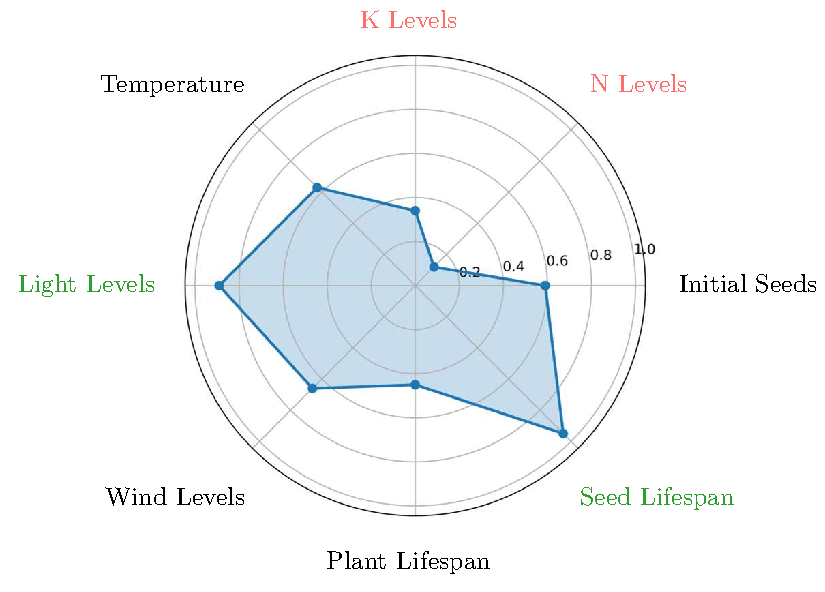
\includegraphics[scale=0.6]{figures/radarchart2.pdf}
    \captionsetup{width=0.9\textwidth}
    \caption{\textbf{Radar chart of model hyperparameters.} The two most impactful factors of our model were light levels and seed lifespan, but nutrient levels were least significant.} 
    \label{fig:radarchart1}
\end{figure}

\subsection{Strengths}

\begin{enumerate}
 \item Our model’s main strength is its ability to \textbf{powerfully generalize}.
    \begin{quote}
        For instance, by including numerous regional and climate hyperparameters into a single, robust framework, our model enables any investigator to thoroughly examine a plot of land for the growth of dandelions. Furthermore, all hyperparameters necessary can be easily obtained from open-access soil samples and climate analysis.
    \end{quote}
\item  Our model employs both \textbf{deterministic and probabilistic} techniques.
\begin{quote}
    Our model reflects real-life behavior of a cyclic dandelion population growth pattern and allows for stochastic variation in dandelion movement and growth.
\end{quote}

\item A thorough Monte Carlo simulation and sensitivity analysis performed \textbf{helps dandelion growers} and harvesting firms best grow dandelions through our analysis of impact factors.
\begin{quote}
    Our analysis concluded that light levels and seed lifespans impact dandelion growth the most; therefore, dandelion harvesters must prioritize these factors above all others to ensure that dandelions can grow most optimally.
\end{quote}
\end{enumerate}

\subsection{Limitations}
\begin{enumerate}
\item Some special data for dandelions could not be found, and so we assumed \textbf{that seeds act as independent agents} and follow growth cycles based on some key climate parameters. 
\begin{quote}
    More abundant data resources can guarantee more robust accommodation for diverse climates in our models. For example, occurrences of natural disasters, significant human interference, and specific consumer-based behaviors would result in a more adept model. 
\end{quote}

\item Our model \textbf{derives climate and death rates from historical data}.
\begin{quote}
    Therefore, our model lacks predictive power for factors such as global warming and competition with other species. Despite this limitation, using stochastic processes ensures that our model tends toward realism while also maintaining model elegance.
\end{quote}
\end{enumerate}

